\section{Schemes}
    \subsection{The Zariski topology and affine schemes}
        \subsubsection{The prime spectrum of a commutative ring} \index{$\Spec$}
            \begin{definition}[Spectra of commutative rings]
                To any commutative ring $R$, let us \textit{contravariantly functorially} associate, first of all, a set $\Spec R$ consisting of all prime ideals of $R$. This is called the spectrum, or the prime spectrum, of $R$. In other words, $\Spec$ is a functor from $\Cring^{\op}$ to $\Sets$.
            \end{definition}
            \begin{remark}[Why is $\Spec$ a contravariant functor ?]
                One can very well construct the theory of affine schemes based on an alternative \textit{covariant} functor $"\Spec": \Cring \to \Sets$, which assigns to a commutative ring its set of prime ideals too. However, this would not have made our lives easy, as the images under ring homomorphisms of a prime ideal is not necessarily prime, whereas the preimage under ring homomorphisms of a prime ideal is always prime. In particular, this means that requiring $\Spec$ to be a contravariant functor ensures that to-be morphisms between affine schemes would always exist, given that the correpsonding morphism between commutative rings exists. In fact, this also proves that $\Spec$ is a well-defined functor, as it guarantees that each commutative ring homomorphism $f: A \to B$ is sent to a \textit{function} $\Spec f$ that maps each element $\q \in \Spec B$ to a unique element $(\Spec f)(\q)$ of $\Spec A$.
            \end{remark}
            \begin{example}[Some interesting underlying sets of ring spectra] \label{example: spectra_sets}
                \noindent
                \begin{enumerate}
                    \item \textbf{(Spectra of fields):} If $k$ is any field, then $\Spec k = \{(0)\}$. To see why this is the case, first of all, let $I$ be an ideal of $k$ that is neither $(0)$ nor $k$. We know that ideals are closed under linear combinations; in this particular instance, $I$ is closed under $k$-linear combinations. Thus, if we view $k$ as a vector space over itself, then $I$ must be a non-zero proper subspace of $k$, since $I$ is a subset of $k$ that is closed under $k$-linear combinations (one could also argue that by the first isomorphism theorem, $I$ is the kernel of some ring homomorphism whose domain is $k$, and we know that kernels are subspaces). Either way, this would mean that:
    					$$0 = \dim_k 0 < \dim_k I < \dim_k k = 1$$
    				and since dimensions of vector spaces are natural numbers, there will be no such natural number $\dim_k I$, i.e. $I$ does not exist. Note that the zero ideal $(0)$ is trivially the zero subspace $0$ of $k$.
    				\item \textbf{(Spectrum of the zero ring):} $\Spec 0 = \varnothing$, because prime ideals are defined to be proper.
    				\item \textbf{(The zero ideal):} The zero ideal is not necessarily prime; as a matter of fact, it is only so inside an integral domain. When zero-divisors are present, say in $\Z/n\Z$ with $n$ composite, the statement:
    				    $$xy \in (0)$$
				    might not imply that $x = y = 0$, but instead, that $x \in (p)$ and $y \in (q)$, with $p, q$ integers such that $pq = n$.
    				\item \textbf{(The complex affine line):} Due to the algebraic closure of $\bbC$, the points of the complex affine line $\A^1_{\bbC} := \Spec \bbC[x]$ (with $t$ some formal variable) are prime ideals of the form $(x - a)$ wherein $a \in \bbC$, along with the prime ideal $(0)$. To see in more details why this is the case, let us first recall because $\bbC$ is a separably closed field, every single-variable polynomial over $\bbC$ splits completely into linear factor. This, along with the fact that $\bbC[x]$ is a PID, tells us that ideals of $\bbC[x]$ are actually all contained in \textit{principal} ideals generated by linear polynomials; note that these principal ideals are prime, precisely because $\bbC$ is separably closed. Lastly. because $\bbC$ is algebraically closed, there is a bijective correspondence between the principal ideals generated by linear polyonomials $(x - a)$ and the individual complex numbers $a \in \bbC$. Thus, the prime ideals of $\bbC[x]$ are either of the form $(0)$ or $(x - a)$, wherein $a \in \bbC$. 
    				\\
    				Below is an illustration by Ravi Vakil of the complex affine line:
    				    \begin{figure}[H]
    				        \centering
    				        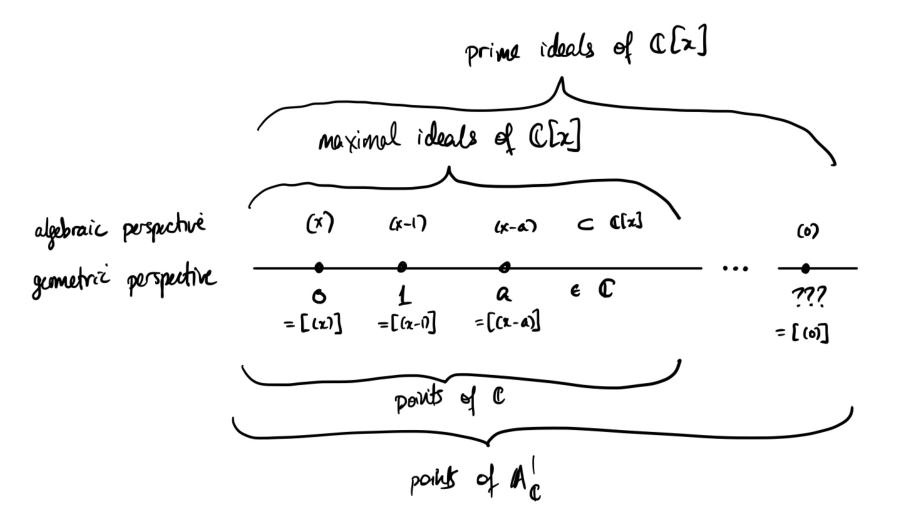
\includegraphics[width=\linewidth,height=\textheight,keepaspectratio]{Figures/complex affine line.png}
    				        \caption{The complex affine line $\A^1_{\bbC}$ (\cite{risingsea}, figure 3.1)}
    				        \label{fig: complex_affine_line}
    				    \end{figure}
    				This result generalises in an obvious manner to algebraically closed fields other than $\bbC$; so for instance, studying schemes over the field $\overline{\Q}$ of algebraic numbers might help one understand more about polynomials with rational coefficients.
    				\item \textbf{(The affine line over a separably closed but not algebraically closed field):} Let $k$ be a field that is separably closed but not algebraically closed (we can take $k = \F_p(t)^{\sep}$, for example). Then, the set of non-zero prime ideals of $\A^1_k$ need not be in bijection with $k$ itself.
    				\item \textbf{(Spectrum of the integers):} The prime ideals of $\Z$ are either generated by prime numbers themselves, or the zero ideal $(0)$. Thus, the set $\Spec \Z$ is in bijection with the \textit{union} of the set of all prime numbers and the set $\{(0)\}$. 
                \end{enumerate}
            \end{example}
        
        \subsubsection{The Zariski topology as a point-set topology} \index{Topology!Zariski}
            \begin{definition}[Zariski-closed subsets] \label{def: zariski_closed}
                Let $R$ be a commutative ring and let $\calF$ be an arbitrary subset of $R$. Then, let us declare that sets of the following form are closed in the to-be Zariski topology:
                    $$V(\calF) := \left\{\p \in \Spec R \mid \p \supset \calF \right\}$$
                When it might be possible to confuse Zariski-closed subsets of different ring spectra, we will write $V_R(\calF)$ instead of simply $V(\calF)$.
            \end{definition}
            \begin{remark}
                Of course, sets of the form $\Spec R \setminus V(\calF)$ are Zariski-open (that is, if we are assuming that the \href{https://ncatlab.org/nlab/show/excluded+middle}{\underline{the Law of Excluded Middle}} holds).
            \end{remark}
            
            \begin{proposition}[Well-definiteness of the Zariski topology] \label{prop: zariski_closed_well_definiteness}
                Let $R$ be an arbitrary commutative ring and assume the Law of Excluded Middle. Then, Zariski-closed subsets as defined in \ref{def: zariski_closed} actually define a topology on $\Spec R$, which of course, is called the Zariski topology.
            \end{proposition}
                \begin{proof}
                    For each subset $\calF$ of $R$, let us write $I(\calF)$ for the $R$-ideal generated by $\calF$. Let us now verify the axioms defining topologies on sets one-by-one.
                        \begin{enumerate}
                            \item \textbf{(The empty set and the whole set are closed):} The empty set is just $V(R)$ and that $\Spec R$ is just $V\left((0)\right)$, which are, by definition, closed in the Zariski topology. Thus, both the empty set and the whole space are Zariski-closed.
                            \item \textbf{(Finite unions of closed sets are closed):} Let $\{V(\calF_{\alpha})\}_{\alpha \in A}$ be a \textit{finite} set of Zariski-closed subsets of $\Spec R$ and consider the following chain of logical \textit{implications} (wherein $\p$ is a prime ideal of $R$, even though this fact can be inferred from the statements themselves):
                                $$
                                    \begin{aligned}
                                        & \p \in \bigcup_{\alpha \in A} V(\calF_{\alpha})
                                        \\
                                        \iff & \exists \alpha \in A: \p \in V(\calF_{\alpha})
                                        \\
                                        \iff & \exists \alpha \in A: \p \supset \calF_{\alpha}
                                        \\
                                        \iff & \bigvee_{\alpha \in A} (\p \supset \calF_{\alpha})
                                        \\
                                        \implies & \forall \left(f_{\alpha}\right)_{\alpha \in A} \in \prod_{\alpha \in A} \calF_{\alpha}: \prod_{\alpha \in A} f_{\alpha} \in \p
                                        \\
                                        \iff & \bigwedge_{\left(f_{\alpha}\right)_{\alpha \in A} \in \prod_{\alpha \in A} \calF_{\alpha}} \left(\prod_{\alpha \in A} f_{\alpha} \in \p\right)
                                        \\
                                        \iff & \p \supset \left\{\prod_{\alpha \in A} f_{\alpha} \: \bigg| \: \forall \alpha \in A: f_{\alpha} \in \calF_{\alpha} \right\}
                                        \\
                                        \iff & \p \in V\left(\left\{\prod_{\alpha \in A} f_{\alpha} \: \bigg| \: \forall \alpha \in A: f_{\alpha} \in \calF_{\alpha} \right\}\right)
                                    \end{aligned}
                                $$
                            wherein the fourth line, in particular, holds due to the fact that ideals, by definition, are closed under scalar multiplication by elements of their ambient rings. Now, to upgrade the fourth line to an equivalence, we can show that:
                                $$\bigwedge_{\left(f_{\alpha}\right)_{\alpha \in A} \in \prod_{\alpha \in A} \calF_{\alpha}} \left(\prod_{\alpha \in A} f_{\alpha} \in \p\right) \implies \bigvee_{\alpha \in A} (\p \supset \calF_{\alpha})$$
                            or, as we have assumed that the Law of Excluded Middle holds, we have the following:
                                $$
                                    \begin{aligned}
                                        & \left(\bigwedge_{\left(f_{\alpha}\right)_{\alpha \in A} \in \prod_{\alpha \in A} \calF_{\alpha}} \left(\prod_{\alpha \in A} f_{\alpha} \in \p\right) \implies \bigvee_{\alpha \in A} (\p \supset \calF_{\alpha})\right)
                                        \\
                                        \vdash & \left(\neg \bigwedge_{\left(f_{\alpha}\right)_{\alpha \in A} \in \prod_{\alpha \in A} \calF_{\alpha}} \left(\prod_{\alpha \in A} f_{\alpha} \in \p\right) \implies  \neg \bigvee_{\alpha \in A} (\p \supset \calF_{\alpha})\right)
                                    \end{aligned}
                                $$
                            meaning that we can prove the contraposition instead. To that end, consider the following:
                                $$
                                    \begin{aligned}
                                        & \neg \bigwedge_{\left(f_{\alpha}\right)_{\alpha \in A} \in \prod_{\alpha \in A} \calF_{\alpha}} \left(\p \ni \prod_{\alpha \in A} f_{\alpha}\right)
                                        \\
                                        \implies & \bigvee_{\left(f_{\alpha}\right)_{\alpha \in A} \in \prod_{\alpha \in A} \calF_{\alpha}} \neg \left(\p \ni \prod_{\alpha \in A} f_{\alpha}\right)
                                        \\
                                        \implies & \bigwedge_{\alpha \in A} \left(\bigvee_{f_{\alpha} \in \calF_{\alpha}} \neg(\p \ni f_{\alpha})\right)
                                        \\
                                        \implies & \bigwedge_{\alpha \in A} \left(\neg \bigwedge_{f_{\alpha} \in \calF_{\alpha}} (\p \ni f_{\alpha})\right)
                                        \\
                                        \implies & \bigwedge_{\alpha \in A} \neg (\p \supset \calF_{\alpha})
                                        \\
                                        \implies & \neg \bigvee_{\alpha \in A} (\p \supset \calF_{\alpha})
                                    \end{aligned}
                                $$
                            Thus, we have managed to show that:
                                $$\neg \bigwedge_{\left(f_{\alpha}\right)_{\alpha \in A} \in \prod_{\alpha \in A} \calF_{\alpha}} \left(\prod_{\alpha \in A} f_{\alpha} \in \p\right) \implies  \neg \bigvee_{\alpha \in A} (\p \supset \calF_{\alpha})$$
                            and therefore:
                                $$\p \in \bigcup_{\alpha \in A} V(\calF_{\alpha}) \iff \p \in V\left(\left\{\prod_{\alpha \in A} f_{\alpha} \: \bigg| \: \forall \alpha \in A: f_{\alpha} \in \calF_{\alpha} \right\}\right)$$
                            Because $\p$ was chosen arbitrarily, this implies that:
                                $$\bigcup_{\alpha \in A} V(\calF_{\alpha}) = V\left(\left\{\prod_{\alpha \in A} f_{\alpha} \: \bigg| \: \forall \alpha \in A: f_{\alpha} \in \calF_{\alpha} \right\}\right)$$
                            Hence, the \textit{finite} union $\bigcup_{\alpha \in A} V(\calF_{\alpha})$ is Zariski-closed by definition, and consequently, all finite unions of Zariski-closed sets are closed in the Zariski topology themselves (since $\{\calF_{\alpha}\}_{\alpha \in A}$ is an arbitrary fintie set of subsets of $R$). Note that the finiteness assumption on the index set $A$ is crucial, as without it, one would not be able to properly make sense of the product $\prod_{\alpha \in A} f_{\alpha}$.
                            \item \textbf{(Intersections of closed sets are closed):} Let $\{V(\calF_{\alpha})\}_{\alpha \in A}$ be an \textit{arbitrary} set of Zariski-closed subsets of $\Spec R$ and consider the following chain of logical equivalences (wherein $\p$ is a prime ideal of $R$, and again, this fact can be deduced from the statements themselves):
                                $$
                                    \begin{aligned}
                                        & \p \in \bigcap_{\alpha \in A} V(\calF_{\alpha})
                                        \\
                                        \iff & \forall \alpha \in A: \p \in V(\calF_{\alpha})
                                        \\
                                        \iff & \forall \alpha \in A: \p \supset \calF_{\alpha}
                                        \\
                                        \iff & \p \supset I\left(\bigcup_{\alpha \in A} \calF_{\alpha}\right)
                                        \\
                                        \iff & \p \in V\left(I\left(\bigcup_{\alpha \in A} \calF_{\alpha}\right)\right)
                                    \end{aligned}
                                $$
                            It tells us that \textit{any} prime ideal $\p$ is in an intersection of Zariski-closed subsets of $\Spec R$ defined by subsets $\calF_{\alpha}$ of $R$ if and only if it is in the Zariski-closed subset of $\Spec R$ defined by the ideal generated by the union of the sets $\calF_{\alpha}$, or in other words, that:
                                $$\bigcap_{\alpha \in A} V(\calF_{\alpha}) = V\left(I\left(\bigcup_{\alpha \in A} \calF_{\alpha}\right)\right)$$
                            In turn, this implies that the intersection of the Zariski-closed sets $V(\calF_{\alpha})$ is itself closed in the Zariski topology, and since the index set $A$ is was chosen arbitrarily, this means that arbitrary intersections of Zariski-closed sets are themselves Zariski-closed.
                        \end{enumerate}
                    Thus, with closed sets as in definition \ref{def: zariski_closed}, the Zariski topology on prime spectra of commutative rings is well-defined.
                \end{proof}
            \begin{corollary}[Quotients are closed] \label{coro: quotients_are_closed}
                Let $R$ be a commutative ring and let $I$ be an $R$-ideal. Then, $\Spec R/I$ is homeomorphic to a Zariski-closed subset of $\Spec R$. 
            \end{corollary}
                \begin{proof}
                    This comes from a straightforward application of the third isomorphism theorem for modules.
                \end{proof}
                
            \begin{definition}[A different approach: Zariski-open sets] \label{def: zariski_open}
                Let $R$ be a commutative ring. Then, let us declare that subsets of $\Spec R$ of the following form are open in the to-be Zariski topology:
                    $$D(f) := \{\p \in \Spec R \mid \p \not \ni f\}$$
                Whenever referring to more than one ring spectra, it might be beneficial to specifically write $D_R(f)$ instead of $D(f)$.
            \end{definition}
            \begin{remark} \label{remark: basic_opens_complements}
                For any commutative ring $R$, one can show through the following logical equivalences that:
                    $$D(f) = \Spec R \setminus V\left((f)\right)$$
                wherein $\p$ is an arbitrary prime ideal of $R$:
                    $$
                        \begin{aligned}
                            & \p \in D(f)
                            \\
                            \iff & \p \in \{\q \in \Spec R \mid \q \not \ni f\}
                            \\
                            \iff & \neg(\p \ni f)
                            \\
                            \iff & \neg(\p \supset (f))
                            \\
                            \iff & \p \in \Spec R \setminus \{\q \in \Spec R \mid \q \supset (f)\}
                            \\
                            \iff & \p \in \Spec R \setminus V\left((f)\right)
                        \end{aligned}
                    $$
            \end{remark}
            
            \begin{proposition}[Well-definiteness of the Zariski topology] \label{prop: zariski_open_well_definiteness}
                Let $R$ be an arbitrary commutative ring and assume the Law of Excluded Middle. Then, Zariski-open subsets as defined in \ref{def: zariski_open} actually define a topology on $\Spec R$, which of course, is called the Zariski topology.
            \end{proposition}
                \begin{proof}
                    Let us verify the axioms defining topologies on sets one-by-one.
                        \begin{enumerate}
                            \item \textbf{(The empty set and the whole set are open):} Consider the set $D(1)$, which by definition, is given by:
                                $$D(1) := \{\p \in \Spec R \mid \p \not \ni 1\}$$
                            Because prime ideals are defined to be proper, and because proper ideals are never (multiplicatively) unital, one gets that:
                                $$D(1) = \Spec R$$
                            In other words, the whole of $\Spec R$ is open by definition. Now, consider the following:
                                $$D(0) := \{\p \in \Spec R \mid \p \not \ni 0\} = \varnothing$$
                            which holds because ideals are submodules of their ambient rings, and modules over rings must contain $0$ (as an additive identity) by definition. Thus, the empty set is also Zariski-open by definition. 
                            \item \textbf{(Unions of open sets are open):} Let $\{f_{\alpha}\}_{\alpha \in A}$ be an \textit{arbitrary} set of elements of $R$ and let us apply remark \ref{remark: basic_opens_complements} to get the following chain of logical equivalences regarding the union of the sets $D(f_{\alpha})$, wherein $\p$ is an \textit{arbitrary} prime ideal of $R$:
                                $$
                                    \begin{aligned}
                                        & \p \in \bigcup_{\alpha \in A} D(f_{\alpha})
                                        \\
                                        \iff & \bigvee_{\alpha \in A} \left(\p \in D(f_{\alpha})\right)
                                        \\
                                        \iff & \bigvee_{\alpha \in A} \neg \left(\p \in V\left((f_{\alpha})\right)\right)
                                        \\
                                        \iff & \neg \bigwedge_{\alpha \in A} \left(\p \in V\left((f_{\alpha})\right)\right)
                                        \\
                                        \iff & \p \in \Spec R \setminus \bigcap_{\alpha \in A} V\left((f_{\alpha})\right)
                                    \end{aligned}
                                $$
                            This shows that:
                                $$\bigcup_{\alpha \in A} D(f_{\alpha}) = \Spec R \setminus \bigcap_{\alpha \in A} V\left((f_{\alpha})\right)$$
                            In proposition \ref{prop: zariski_closed_well_definiteness}, we have already shown using only definition \ref{def: zariski_closed} that arbitrary intersections of Zariski-closed sets are Zariski-closed themselves; in particular, this means that $\bigcap_{\alpha \in A} V\left((f_{\alpha})\right)$ is Zariski-closed. Then, by using the Law of Excluded Middle, one can see that the complement $\Spec R \setminus \bigcap_{\alpha \in A} V\left((f_{\alpha})\right)$ is necessarily Zariski-open. Thus, arbitrary unions of Zariski-open sets are Zariski-open themselves.
                            \item \textbf{(Finite intersections of open sets are open):} Let $\{f_{\alpha}\}_{\alpha \in A}$ be an \textit{finite} set of elements of $R$ and consider the following chain of logical equivalences regarding the union of the sets $D(f_{\alpha})$, wherein $\p$ is a prime ideal of $R$:
                                $$
                                    \begin{aligned}
                                        & \neg \left(\p \in \bigcap_{\alpha \in A} D(f_{\alpha})\right)
                                        \\
                                        \iff & \neg \bigwedge_{\alpha \in A} \left(\p \in D(f_{\alpha})\right)
                                        \\
                                        \iff & \bigvee_{\alpha \in A} \neg \left(\p \in D(f_{\alpha})\right)
                                        \\
                                        \iff & \bigvee_{\alpha \in A} \left(\p \in \Spec R \setminus D(f_{\alpha})\right)
                                        \\
                                        \iff & \bigvee_{\alpha \in A} \left(\p \in V\left((f_{\alpha})\right)\right)
                                        \\
                                        \iff & \p \in \bigcup_{\alpha \in A} V\left((f_{\alpha})\right)
                                    \end{aligned}
                                $$
                            (let us note that the fifth line holds thanks to remark \ref{remark: basic_opens_complements}). Now, the contraposition of the equivalence:
                                $$\neg \left(\p \in \bigcap_{\alpha \in A} D(f_{\alpha})\right) \iff \p \in \bigcup_{\alpha \in A} V\left((f_{\alpha})\right)$$
                            is:
                                $$\neg \neg \left(\p \in \bigcap_{\alpha \in A} D(f_{\alpha})\right) \iff \neg \left(\p \in \bigcup_{\alpha \in A} V\left((f_{\alpha})\right) \right)$$
                            From this, one gets the following proof:
                                $$
                                    \begin{aligned}
                                        & \neg \neg \left(\p \in \bigcap_{\alpha \in A} D(f_{\alpha})\right) \iff \neg \left(\p \in \bigcup_{\alpha \in A} V\left((f_{\alpha})\right) \right)
                                        \\
                                        \vdash & \left(\p \in \bigcap_{\alpha \in A} D(f_{\alpha})\right) \iff \left(\p \in \Spec R \setminus \bigcup_{\alpha \in A} V\left((f_{\alpha})\right) \right) 
                                        \\
                                        \vdash & \left(\bigcap_{\alpha \in A} D(f_{\alpha}) = \Spec R \setminus \bigcup_{\alpha \in A} V\left((f_{\alpha})\right)\right)
                                    \end{aligned}
                                $$
                            Lastly, let us recall that by \ref{prop: zariski_closed_well_definiteness}, the \textit{finite} union $\bigcup_{\alpha \in A} V\left((f_{\alpha})\right)$ of Zariski-closed sets is Zariski-closed itself, meaning that by the Law of Excluded Middle, the complement $\Spec R \setminus \bigcup_{\alpha \in A} V\left((f_{\alpha})\right)$ must be Zariski-open. Thus, the union $\bigcap_{\alpha \in A} D(f_{\alpha})$ is Zariski-open. Note that the finiteness assumption on the index set $A$ is crucial, as otherwise, the union $\bigcup_{\alpha \in A} V\left((f_{\alpha})\right)$ might not be Zariski-closed.
                        \end{enumerate}
                    Thus, with open sets as in definition \ref{def: zariski_open}, the Zariski topology on prime spectra of commutative rings is well-defined.
                \end{proof}
            
            \begin{proposition}[Unifying the two definitions] \label{prop: zariski_topology_equivalence}
                By asuming the Law of Excluded Middle, one gets the same topology on spectra of commutative rings via the approaches presented in definitions \ref{def: zariski_closed} and \ref{def: zariski_open}.
            \end{proposition}
                \begin{proof}
                    Let $R$ be a commutative ring. It is sufficient to show that for each element $f \in R$, the complement $\Spec R \setminus D(f)$ is closed in the sense of definition \ref{def: zariski_closed}, or equivalently, for each subset $\calF \subset R$, the complement $\Spec R \setminus V(\calF)$ is open in the sense of definition \ref{def: zariski_open}. We will be attempting the second approach. To that end, let us directly the following chain of logical equivalences:
                        $$
                            \begin{aligned}
                                & \p \in \bigcup_{\alpha \in A} D(f_{\alpha})
                                \\
                                \iff & \exists \alpha \in A: \p \in D(f_{\alpha})
                                \\
                                \iff & \exists \alpha \in A: \p \in \{\q \in \Spec R \mid \q \not \ni f_{\alpha}\}
                                \\
                                \iff & \exists \alpha \in A: \p \not \ni f_{\alpha}
                                \\
                                \iff & \bigvee_{\alpha \in A} \neg\left(\p \ni f_{\alpha}\right)
                                \\
                                \iff & \neg \bigwedge_{\alpha \in A} (\p \ni f_{\alpha}) 
                                \\
                                \iff & \neg \left(\p \supset \bigcup_{\alpha \in A} \{f_{\alpha}\}\right)
                                \\
                                \iff & \neg \left(\p \supset \{f_{\alpha}\}_{\alpha \in A}\right)
                                \\
                                \iff & \p \in \Spec R \setminus \left\{\q \in \Spec R \mid \q \supset \{f_{\alpha}\}_{\alpha \in A}\right\}
                                \\
                                \iff & \p \in \Spec R \setminus V\left(\{f_{\alpha}\}_{\alpha \in A}\right)
                            \end{aligned}
                        $$
                    Thus:
                        $$\bigcup_{\alpha \in A} D(f_{\alpha}) = \Spec R \setminus V\left(\{f_{\alpha}\}_{\alpha \in A}\right)$$
                    i.e. the complement of the Zariski-closed set $V\left(\{f_{\alpha}\}_{\alpha \in A}\right)$ inside $\Spec R$ is a union of Zariski-open sets $D(f_{\alpha})$, which we know from proposition \ref{prop: zariski_open_well_definiteness} to be Zariski-open itself. As stated, this implies that definitions \ref{def: zariski_closed} and \ref{def: zariski_open} give us the same Zariski topology on prime spectra of commutative rings.
                \end{proof}
            \begin{corollary} \label{coro: zariski_basis}
                Let $R$ be a commutative ring and let $f$ denote elements of $R$. Then, the distinguished Zariski-open sets $D(f)$ form a base of the Zariski topology on $\Spec R$.
            \end{corollary}
                \begin{proof}
                    This is a direct consequence of the fact that complements of Zariski-closed sets are unions of Zariski-open sets of the form $D(f)$.
                \end{proof}
            
            We have managed to show that on each ring spectrum, there is a canonical topology, namely the Zariski topology. A naturaly follow-up question is thus: can we upgrade $\Spec$ to a functor whose domain is $\Top$ instead of $\Sets$ ? Luckily, the answer is yes, although we will need to do some work to show that this is the case. 
            \begin{proposition}[Continuous functions between spectra] \label{prop: continuous_functions_between_spectra}
                By equipping prime spectra of commutative rings with the Zariski topology (in either the sense of definition \ref{def: zariski_closed} or \ref{def: zariski_open}), one naturally gets a functor:
                    $$\Spec: \Cring^{\op} \to \Top$$
                assigning to commutative rings their respective Zariski topological spaces.
            \end{proposition}
                \begin{proof}
                    It will suffice to show that given any ring homomorphism $f: A \to B$, the induced map $\Spec f: \Spec B \to \Spec A$ is continuous, which we can do by showing that preimages of Zariski-open subsets of $\Spec A$ under $\Spec f$ are closed in $\Spec B$; in fact, we can restrict our attention to \textit{basic} open subsets of $\Spec A$ (i.e. subsets of the form $D_A(a)$, for some $a \in A$), as they form a basis for the Zariski topology on $\Spec A$. Let $D_A(a)$ be such a basic open set. It preimage under $\Spec f$ is thus the following subset of $\Spec B$:
                        $$(\Spec f)^{-1}\left(D_A(a)\right) = \{\q \in \Spec B \mid (\Spec f)(\q) \in D_A(a)\}$$
                    Writing out the definition of $D_A(a)$ (cf. definition \ref{def: zariski_open}) then gives the following chain of logical equivalences:
                        $$
                            \begin{aligned}
                                & \q \in (\Spec f)^{-1}\left(D_A(a)\right)
                                \\
                                \iff & (\Spec f)(\q) \in D_A(a)
                                \\
                                \iff & f^{-1}(\q) \in D_A(a)
                                \\
                                \iff & \neg(f^{-1}(\q) \ni a)
                                \\
                                \iff & \neg(\q \ni f(a))
                                \\
                                \iff & \q \in D_B(f(a))
                            \end{aligned}
                        $$
                    which proves that:
                        $$(\Spec f)^{-1}\left(D_A(a)\right) = D_B(f(a))$$
                    and because $D_B(f(a))$ is open by definition, so is the preimage $(\Spec f)^{-1}(D_A(a))$. As stated at the beginning, this implies that $\Spec f$ is a continuous function, and thus there exists a functor:
                        $$\Spec: \Cring^{\op} \to \Top$$
                    assigning commutative rings and homomorphisms between them to ring spectra equipped with the Zariski topology and continuous maps in between.
                \end{proof}
                
            \begin{example}[Topologically interesting ring spectra]
                \noindent
                \begin{enumerate}
                    \item \textbf{(The complex affine plane and complex affine $n$-spaces):}
                        \begin{figure}[H]
                            \centering
                            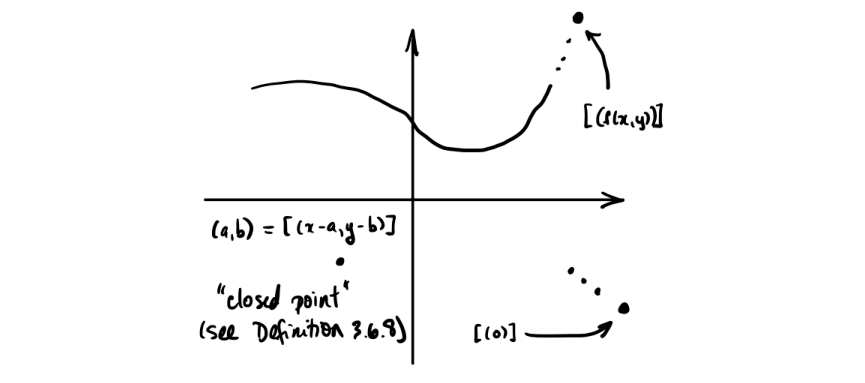
\includegraphics[width=\linewidth,height=\textheight,keepaspectratio]{Figures/complex affine plane.png}
                            \caption{The complex affine plane $\A^2_{\bbC}$ (\cite{risingsea}, figure 3.3)}
                            \label{fig: complex_affine_plane}
                        \end{figure}
                    \item \textbf{(Revisiting $\Spec \Z$):}
                        \begin{figure}[H]
                            \centering
                            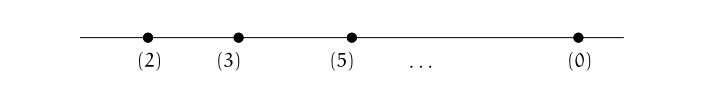
\includegraphics[width=\linewidth,height=\textheight,keepaspectratio]{Figures/Spec Z.png}
                            \caption{$\Spec \Z$ (\cite{risingsea}, figure 3.2)}
                            \label{fig: Spec_Z}
                        \end{figure}
                    \item \textbf{(A conic):}
                        \begin{figure}[H]
                            \centering
                            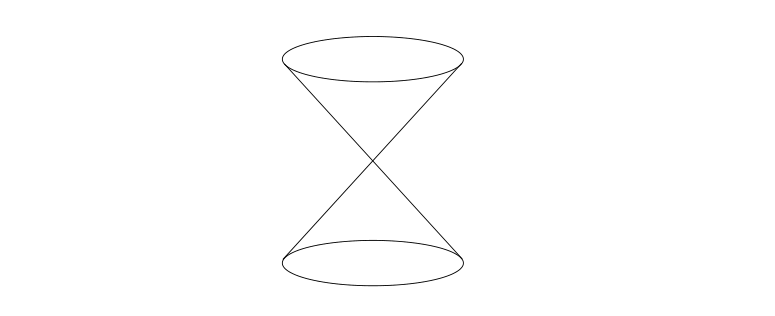
\includegraphics[width=\linewidth,height=\textheight,keepaspectratio]{Figures/conic.png}
                            \caption{A conic which is Zariski-closed inside $\A^3_{\bbC}$ (\cite{risingsea}, figure 3.4)}
                            \label{fig: conic}
                        \end{figure}
                \end{enumerate}
            \end{example}
            
            \begin{remark}[Comparing $\Spec$ and $\Spm$]
                Historically (and only because mathematicians were more interested in complex algebraic geometry back in the days), it was not the set of prime ideals of a commutative ring that was considered, but rather, the set of \textit{maximal} ideals. This was not out of \textit{na\"ivet\'e}, though. Maximal ideals enjoy being closed points in prime spectra of commutative rings (one can prove this by first looking at varieties $V(\m)$ associated to maximal ideals $\m$ of some commutative ring $R$, and then applying the definition of the (underlying set of) these varieties as spaces whose points are prime ideals containing $\m$, and then lastly, applying the usual definition of topological closures; as a corollary, one gets that prime ideals that are not maximal get sent by $\Spec$ to non-closed points in $\Spec R$), and so doing geometry with them is a lot more intuitive (albeit more restrictive as well) then doing so with all prime ideals. For instance, the underlying set of $\Spm \bbC[x]$ is precisely $\bbC$, whereas that of $\Spec \bbC[x]$ can be thought of as $\bbC \cup \{\infty\}$, i.e. as the Riemann sphere; in particular, the zero ideal $(0)$ corresponds to the point \say{at infinity}, which we denote by $\infty$. 
            \end{remark}
            
            \begin{example}[Non-isomorphic rings with homeomorphic spectra] \label{example: nonisomorphic_rings_with_the_same_spectra}
                The following examples are of non-isomorphic rings with homeomorphic prime spectra; through them, we are able to show that the functor $\Spec: \Cring^{\op} \to \Top$ is not an equivalence of categories (nor even a fully faithful inclusion). 
                \begin{enumerate}
                    \item \textbf{(Fields):} The prime spectra of any field is just the one-point space, but clearly, not all fields are isomorphic.
                    \item \textbf{(Discrete valuation rings):} The spectrum of any \href{https://en.wikipedia.org/wiki/Discrete_valuation_ring}{\underline{discrete valuation ring}} is homeomorphic to the \href{https://ncatlab.org/nlab/show/Sierpinski+space}{\underline{Sierpi\'nski space}} (to see why this is the case, firstly check that discrete valuation rings only have two prime ideals, one being the zero ideal and one being the unique maximal ideal, and that the latter is a closed point in the spectrum whereas the former is generic), but of course, not all discrete valuation rings are isomorphic to one another.
                \end{enumerate}
            \end{example}
        
        \subsubsection{Affine schemes}
            Next, we will be discussing the idea of so-call \textbf{structure sheaves}, but in order to make sense of these entities, we will need to know what $\C$-valued sheaves are for categories $\C$ more general than $\Sets$:
            \begin{definition}[$\C$-valued sheaves] \label{def: C_valued_sheaves}
                \noindent
                \begin{enumerate}
                    \item \textbf{($\C$-valued sheaves):} Let $(\S, J)$ be a site\footnote{... which is not necessarily small, as cases such as $\S \cong \Top$ and $\S \cong \Mfd^{\smooth}_{/\R}$ are interesting in their own rights.} and let $\C$ be a category with \textit{enough small limits} and \textit{enough filtered colimits} (the purpose of the second hypothesis is to ensure that stalks, should they exist, are well-defined); note that $\C$ need not be small. Additionally, fix an \textit{arbitrary} object $x$ of $\S$ along with a covering sieve $\calU_{/x} \in J$ thereon. Also, let $j: \S \to \Psh_{\C}(\S)$ be the Yoneda embedding. Then, a \textbf{$\C$-valued sheaf} on $(\S, J)$ is a functor $\calF: \S^{\op} \to \C$ such that $\calF(x) \cong \calF\left( \underset{u \in \calU_{/x}}{\colim} ju \right)$.
                    \item \textbf{($\C$-topoi):} $\C$-valued sheaves on a given site $(\S, J)$ form a category in the obvious manner. We shall be writing $\Sh_{\C}(\S, J)$ for this category, and such categories will be called \textbf{$\C$-topoi}, even though this is an abuse of terminology.
                \end{enumerate}
            \end{definition}
            \begin{example}[Sheaves of rings]
                The notion of sheaves of rings, which subsumes that of structure sheaves (cf. proposition \ref{prop: structure_sheaf}), follows suite from definition \ref{def: C_valued_sheaves}. Note that such constructions are well-defined, as the category of rings is both complete and cocomplete.
            \end{example}
            
            Having defined sheaves that might take values categories other than $\Sets$, let us now try to define affine schemes as locally ringed spaces whose underlying topological spaces are spectra of commutative rings, and whose structure presheaves have a certain condition imposed upon them, which happens to guarantee that:
                \begin{enumerate}
                    \item these structure presheaves are indeed sheaves (proposition \ref{prop: structure_sheaf}) with local stalks (corollary \ref{coro: structure_sheaf_properties}), and
                    \item they are unique (proposition \ref{prop: structure_sheaf_uniqueness}), which is an important feature, because ringed spaces are uniquely defined by their structure sheaves; this fact will also be used to establish the fully faithfulness of $\Spec$ as a functor from $\Cring^{\op}$ to the category $\Loc\Ringed\Spc$ of locally ringed spaces. 
                \end{enumerate}
            Our efforts will culminate in definition \ref{def: affine_schemes}.
                
            \begin{proposition}[Structure sheaves of affine schemes] \label{prop: structure_sheaf} \index{Structure sheaves}
                Let $k$ be a base commutative ring, and let $\calO_{\Spec R}$ be \textit{a} presheaf of commutative rings on $\Ouv(\Spec R)$ determined by the following rule on objects:
                    $$\calO_{\Spec R}(D_R(f)) \cong R_f$$
                for all element $f \in R$. Any presheaf on $\Ouv(\Spec R)$ that are defined this way is a Zariski sheaf (i.e. a sheaf on the site $\Ouv(\Spec R)$ of Zariski-open subsets of $\Spec R$), and is called \textit{a} \textbf{structure sheaf} on $\Spec R$.
            \end{proposition}
            \begin{corollary}[On the locality of stalks] \label{coro: structure_sheaf_properties}
                Let $R$ be a commutative ring and let $\p$ be an arbitrary prime ideal of $R$. Then one has the following characterisation of the stalk $\calO_{\Spec R, \p}$ at $\p$ of the structure sheaf $\calO_{\Spec R}$:
                    $$\calO_{\Spec R, \p} \cong R_{\p}$$
                This shows that affine schemes are, in fact, \textit{locally} ringed spaces and not just ringed spaces. 
            \end{corollary} 
                \begin{proof}
                    Recall that the stalk $\calF_x$ of a sheaf (of sets) $\calF$ on a topological space $(X, \Ouv(X))$ is given by the filtered colimit indexed by the poset of open neighbourhoods of the chosen point $x \in X$:
                        $$\calF_x \cong \underset{U \in \{V \in \Ouv(X) \mid V \ni x\}}{\colim} \calF(U)$$
                    By adapting this definition to the underlying Zariski-topological spaces of affine schemes, we get that:
                        $$\calO_{\Spec R, \p} \cong \underset{U \in \{V \in \Ouv(\Spec R) \mid V \ni \p\}}{\colim} \calO_{\Spec R}(U)$$
                    with $\Ouv(\Spec R)$ the Zariski topology defined via open sets as in definition \ref{def: zariski_open}. In corollary \ref{coro: zariski_basis}, we have already seen how the distinguished Zariski-open sets defined in definition \ref{def: zariski_open} form a basis for the Zariski topology on commutative ring spectra, and so the above filtered colimit can be rewritten as:
                        $$\calO_{\Spec R, \p} \cong \underset{D_R(f) \in \{V \in \Ouv(\Spec R) \mid V \ni \p\}}{\colim} \calO_{\Spec R}\left(D_R(f)\right)$$
                    and because $D_R(f) = \{\p \in \Spec R \mid \p \not \ni f\}$, one subsequently gets:
                        $$\calO_{\Spec R, \p} \cong \underset{f \in \{g \in R \mid g \not \in \p\}}{\colim} \calO_{\Spec R}\left(D_R(f)\}\right)$$
                    Lastly we have the following isomorphism:
                        $$\calO_{\Spec R, \p} \cong \underset{f \in \{g \in R \mid g \not \in \p\}}{\colim} \calO_{\Spec R}\left(D_R(f)\right) \cong \underset{f \in R \setminus \p}{\colim} R_f \cong R_{\p}$$
                    Thus $\calO_{\Spec R, \p} \cong R_{\p}$ as claimed.
                \end{proof}
                
            \begin{proposition}[Uniqueness of structure sheaves] \label{prop: structure_sheaf_uniqueness}
                Let $R$ be a commutative ring. Then, there is only one unique structure sheaf attached to $\Spec R$. 
            \end{proposition}
                \begin{proof}
                    Suppose to the contrary that there exist two \textit{distinct} Zariski sheaves of $R$-algebras on $R\-\Comm\Alg^{\op}$ $\calF$ and $\calG$ such that:
                        $$\forall f \in R: \calF(\Spec R_f) \cong \calG(\Spec R_f) \cong R_f$$
                    However, the localisation of any commutative at its multiplicative identity is just itself, and so:
                        $$\calF(\Spec R) \cong \calG(\Spec R) \cong R$$
                    for all commutative rings $R$. This means that the functors $\calF$ and $\calG$ are naturally isomorphic, i.e. they can not be distinct. Thus, the structure sheaf attached to a given ring spectrum is unique (up to natural isomorphisms, of course).
                \end{proof}
                
            \begin{example}[Spotting structure sheaves in the wild]
                Let $R$ be a discrete valuation ring that is a \href{https://en.wikipedia.org/wiki/Dedekind_domain}{\underline{Dedekind domain}} (so the only proper ideals of $R$ would be $(0)$ and its unique maximal ideal) with unique maximal ideal $\p$, and recall that its spectrum is (homeomorphic to) the Sierpi\'nski space (see example \ref{example: nonisomorphic_rings_with_the_same_spectra} for more details); in particular, the subset $\{(0)\}$ of $\Spec R = \{(0), \p\}$ is the only non-empty open proper subset. Now, suppose that $\calF$ is a Zariski sheaf on $\Spec R$ given by the following formula:
                    $$
                        \calF(U) \cong 
                        \begin{cases}
                            \text{$R$ if $U = \Spec R$}
                            \\
                            \text{$\Frac R$ if $U = \{(0)\}$}
                        \end{cases}
                    $$
                (note that discrete valuation rings are integral domains, so it makes sense to consider their fields of fractions). The point that is to be made here is that $\calF$ qualifies as a structure sheaf on $\Spec R$. To see why this is the case, note that because $R$ has only two prime ideals, namely $(0)$ and $\p$, 
            \end{example}
            
            \begin{example}[The complex affine line]
                Recall that in example \ref{example: spectra_sets}, we have seen how a point of the complex affine line $\A^1_{\bbC}$ is either the zero ideal, or of the form $(t - a)$ for any complex number $a$; one should keep the following picture in mind:
                    \begin{figure}[H]
				        \centering
				        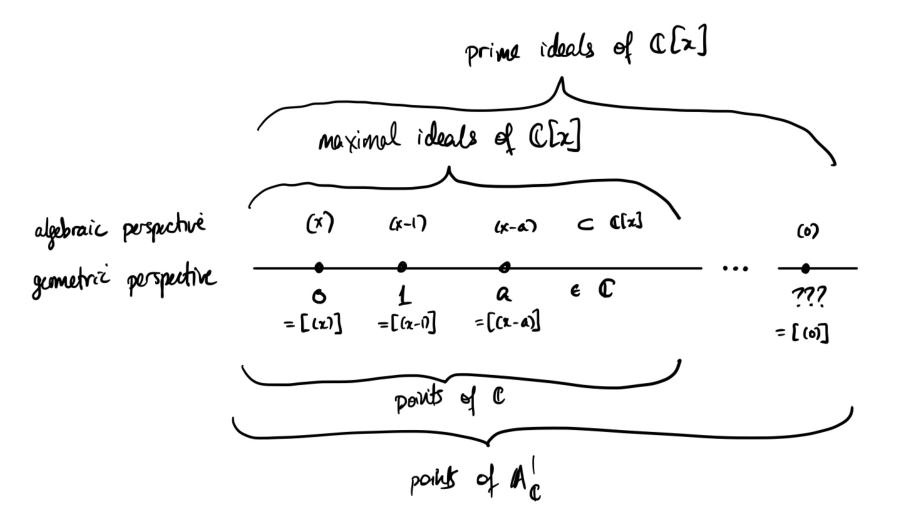
\includegraphics[width=\linewidth,height=\textheight,keepaspectratio]{Figures/complex affine line.png}
				        \caption{The complex affine line $\A^1_{\bbC}$ (\cite{risingsea}, figure 3.1)}
				        \label{fig: complex_affine_line_stalks}
				    \end{figure}
			    \noindent
			    Now, as an affine scheme, $\A^1_{\bbC}$ comes equipped with a structure sheaf $\calO_{\A^1_{\bbC}}$, whose stalks, as shown in corollary \ref{coro: structure_sheaf_properties}, are precisely the localisations of $\bbC[t]$ at its prime ideals. There are thus two cases:
			        \begin{enumerate}
			            \item The stalk at $(0)$ is given by:
			                $$\calO_{\A^1_{\bbC}, (0)} \cong \bbC[t]_{(0)} \cong \bbC(t)$$
		                and thus the residue field is trivially $\bbC(t)$.
			            \item At non-zero primes, the stalks of the structure sheaf $\calO_{\A^1_{\bbC}}$ are given by the following localisations:
			                $$\calO_{\A^1_{\bbC}, (t - a)} \cong \bbC[t]_{(t - a)}$$
		                whose elements we note to be fractions of the form $\frac{f(t)}{g(t)}$ whose denominators do not vanish at $t = a$. Now, recall that the localisation of any commutative ring at a prime ideal is a local ring, and that inside \textit{any} local commutative ring, elements in the complement of the unique maximal ideal are units; in particular, these facts imply that the elements of the complement $\bbC[t]_{(t - a)} \setminus (t - a)\bbC[t]_{(t - a)}$ are all invertible. Consequently, these elements must be fractions $\frac{f(t)}{g(t)}$ whose numerators and denominators both do not vanish at $t = a$. Thus, a reasonable description of the canonical quotient map is the evaluation map:
		                    $$\frac{f(t)}{g(t)} \mapsto \frac{f(a)}{g(a)}$$
	                    whose image is precisely $\bbC$. Therefore, the stalks of $\calO_{\A^1_{\bbC}}$ are all isomorphic to $\bbC$.
			        \end{enumerate}
            \end{example}
        
            \begin{definition}[Affine schemes] \label{def: affine_schemes}
                An \textbf{affine scheme} is a locally ringed space that is isomorphic to one of the form $(|\Spec R|, \calO_{\Spec R})$ for some commutative ring $R$. Morphisms of affine schemes are morphisms of locally ringed spaces, and as such, one has a full subcategory $\Sch^{\aff}$ of affine schemes within the category of locally ringed spaces. 
            \end{definition}
            
            \begin{theorem}[Isbell Duality for locally ringed spaces] \label{theorem: isbell_duality_for_locally_ringed_spaces}
                There is an adjunction as follows:
                    $$
                        \begin{tikzcd}
                        	{\Cring^{\op}} & \Loc\Ringed\Spc
                        	\arrow[""{name=0, anchor=center, inner sep=0}, "\Spec"', bend right, from=1-1, to=1-2]
                        	\arrow[""{name=1, anchor=center, inner sep=0}, "\Gamma"', bend right, from=1-2, to=1-1]
                        	\arrow["\dashv"{anchor=center, rotate=-90}, draw=none, from=1, to=0]
                        \end{tikzcd}
                    $$
            \end{theorem}
            \begin{corollary}
                The adjunction from theorem \ref{theorem: isbell_duality_for_locally_ringed_spaces} restricts down to an adjoint equivalence $\Sch^{\aff} \cong \Cring^{\op}$.
            \end{corollary}

    \subsection{The category of schemes}
        \subsubsection{Schemes}
            \begin{definition}[Schemes] \label{def: schemes}
                A \textbf{scheme} is a locally ringed space $(|X|, \calO_X)$ such that every point $x \in |X|$ as a Zariski-open neighbourhood $U_x \ni x$ that is isomorphic to an affine scheme. Morphisms of schemes are nothing but morphisms of locally ringed spaces, meaning that schemes form a category $\Sch$ which embeds fully faithfully into the category of locally ringed spaces.
            \end{definition}
            
            \begin{proposition}[Open subschemes are open locally ringed subspaces] \label{prop: open_subschemes_are_open_locally_ringed_subspaces}
                Let $X$ be a scheme and let $U \subseteq X$ be an open locally ringed subspace. Then, $U$ will be an open subscheme of $X$. 
            \end{proposition}
                \begin{proof}
                    
                \end{proof}
            \begin{corollary}[Zariski-bases of schemes] \label{coro: zariski_bases_of_schemes}
                
            \end{corollary}
    
        \subsubsection{Properties of schemes and their morphisms}
        
        \subsubsection{Topologies on schemes; descent-theoretic results}
    
    \subsection{Varieties}